%%%%%%%%%%%%%%%%%%%%%%%%%%%%%%%%%%%%%%%%%%%%%%%%%%%%%%%%%%%%%%%%%%%%%%%%
%                                                                      %
%     File: Thesis_Implementation.tex                                  %
%     Tex Master: Thesis.tex                                           %

%%%%%%%%%%%%%%%%%%%%%%%%%%%%%%%%%%%%%%%%%%%%%%%%%%%%%%%%%%%%%%%%%%%%%%%%

\chapter{Interoperability}
\label{chapter:interoperability}
\section{Overview}
\label{section:overview}
Resources need to interact to accomplish collaboration, either designed or emergent. This necessarily entails some
form of mutual knowledge and understanding, but this creates dependencies on other resources that may hamper resource
evolution and that's why Interoperability, a necessary condition to achieve integration between different systems.
Another important factor for integration between systems is decoupling which says that resources need to be independent
to evolve freely and dynamically. Unfortunately, independent resources do not understand each other and are not able to
interact. Therefore, the fundamental problem of resource integration is to provide the maximum decoupling possible while
ensuring the minimum interoperability requirements.

%%%%%%%%%%%%%%%%%%%%%%%%%%%%%%%%%%%%%%%%%%%%%%%%%%%%%%%%%%%%%%%%%%%%%%%%
\section{Interoperability in SOA and REST}
\label{section:InteroperabilitySOAREST}

Currently, enterprise integration is based on SOA and REST; the two most used architectural styles for distributed
interoperability. These styles use symmetric arrangement in which a sender produces a message according to some schema
and the receiver uses the same schema to validate and to get the contents of the message. The message is sent over a
channel between sender and receiver. In SOA web services, schema is usual in XML Schema and WSDL. In the REST world,
schemas are known as media types but perform the same role. The difference is that, instead of being declared in a
separate document referenced by messages, they need to be previously known to the interaction resources, either by
being standard or by having been previously agreed. In any case, the schema or media type must be the same at both
sender and receiver and therefore imposes coupling between the resources for all its possible values, even if only a
few are actually used. In either case, data types need to be fully known by both interacting resources.

 \begin{figure}[!htb]
   \centering
   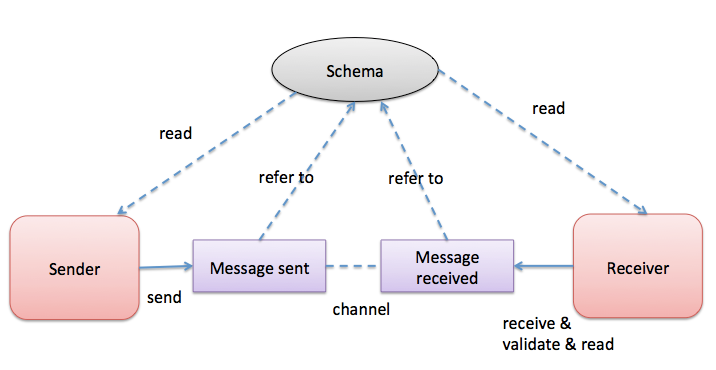
\includegraphics[width=0.9\textwidth]{Figures/schema.png}
   \caption[Interoperability in SOA and REST.]{Interoperability in SOA and REST.}
   \label{fig:interoperability}
 \end{figure}

 \section{Asymmetric interoperability}
 \label{section:AsymmetricInteroperability}

In our solution, we show how interaction is stil possible with only a partial knowledge of types, as long as the
characteristics actually used are included (partial interoperability). This is a way of getting closer to solving the
fundamental integration problem, by reducing coupling to what is actually required.\\

Coupling is thus a necessary bad, without it no interaction is possible. Our goal is to minimize it as much as
possible, down to the minimum level that ensures the level of interaction required by the resources to integrate.\\

In this solutution we will show different approach, based on compliance. Messages do not obey some external schema.
Each message has one specific value which are structured or primitive with its own exclusive schema that is nothing more than a self-description,
without the value variability that a type exhibits. This value and its description can be validated against an infinite number of schemas, those
that have this particular value included in the set of their instances.\\
\begin{figure}[!htb]
  \centering
  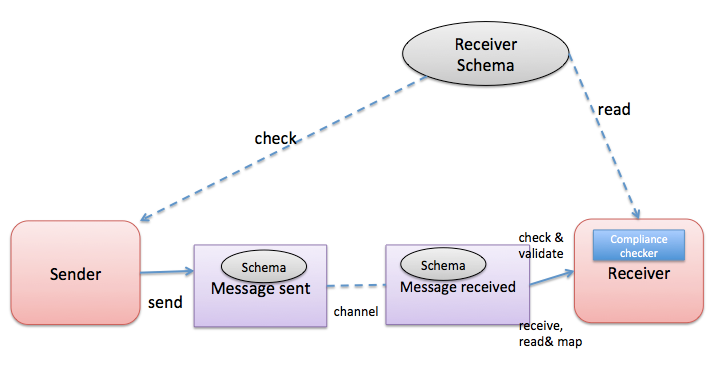
\includegraphics[width=0.9\textwidth]{Figures/asyc.png}
  \caption[Asymmetric interoperability.]{Asymmetric interoperability.}
  \label{fig:Asymmetric}
\end{figure}
The receiver in Figure ~\ref{fig:Asymmetric} exposes a schema that defines the values it is willing to accept.
When a message is received, its internal schema is checked against the receiver’s own schema. If it complies which
means satisfies all the requirements of the receiver’s schema, the message can be accepted and processed. The advantage of this is that a
resource can send a message to all the resources with schemas that the message complies with and, conversely, a
resource can receive messages from any resource that sends messages compliant with its receiving schema.

In other words, coupling occurs only in the characteristics actually used by messages and not in all the characteristics of the schemas used to generate the message or to describe the service of the receiving resource. Since the schemas of
the message and of the receiver are not agreed beforehand, they need to be checked structurally. Resources of primitive
types have predefined compliance rules. Structured resources are compared by the names of components (regardless of
order of declaration or appearance) and (recursively) by the compliance between structured resources with matching
names. Since the order of appearance of named component resources may different in the message and in the receiving
schema, there is the need to map one onto the other. This is a form of polymorphism that increases the range of
applicability of both sender and receiver, constituting a means to reduce coupling to only what is actually used.
Sender and receiver no longer need to be designed for each other but, as long as compliance is ensured, one resource
can replace another. In this case, what is involved is conformance between the replacement and the resource
replaced, stating that the former supports all the characteristics supported by the latter. When a resource is able to
interact with another, although not entirely interoperable with it, we say that have partial interoperability

\begin{figure}[!htb]
  \centering
  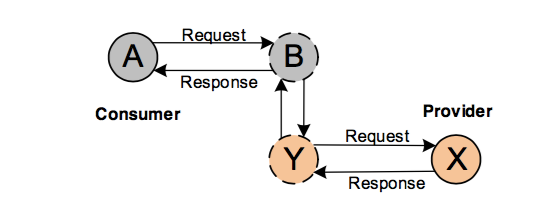
\includegraphics[width=0.9\textwidth]{Figures/partial.png}
  \caption[Partial interoperability, based on compliance and conformance.]{Partial interoperability, based on compliance and conformance.}
  \label{fig:Partial}
\end{figure}

Figure ~\ref{fig:Partial} illustrates these concepts and differentiates compliance from conformance. It also describes complete
transactions, with both request and response. The interacting resources now perform the roles of consumer who makes the request and provider, with sender and receiver roles reversed from request to response.

Interoperability of a consumer with a provider is possible by satisfying the following properties:

Compliance\citep{compliance:def} which means that the consumer must satisfy (comply with) the requirements established
by the provider to accept requests sent to it, without which these cannot be honored.

Conformance\citep{comformance:def2} which means that the provider must fulfill the expectations of the consumer
regarding the effects of a request (including eventual responses), therefore being able to take the form
of (to conform to) whatever the consumer expects it to be.


In full interoperability, the consumer can use all the characteristics that the provider exposes.
This is what happens when schemas are shared. In partial interoperability, the consumer uses only a subset of
those characteristics, which means that compliance and conformance need only be ensured for that subset.
These properties are not commutative (e.g., if P complies with Q, Q does not necessarily comply with P), since the
roles of consumer and provider are different and asymmetric by nature, but are transitive (e.g., if P complies with
Q and Q complies with R, then P complies with R)

In Figure ~\ref{fig:Partial} , a resource A, in the role of consumer, has been designed for full interoperability
with resource B, in the role of provider. A uses only the characteristics that B offers and B offers only the
characteristics that A uses. Let us assume that we want to change the provider of A to resource X, which has been
designed for full interoperability with resource Y, in the role of consumer. The problem is that A was designed to
interact with provider B and X was designed to expect consumer Y. This means that, if we use resource X as a
provider of A, B is how A views provider X and Y is how X views consumer A. Ensuring that A is interoperable with
X requires two conditions such as Compliance and Conformance.
For Compliance; B must comply with Y. Since A complies with B and Y complies with X, this means that A complies with
X and, therefore, A can use X as if it were B, as it was designed for;

For Conformance: Y must conform to B. Since X conforms to Y and B conforms to A, this means that X conforms to
A and, therefore, X can replace (take the form of) B without A noticing it.
 Partial interoperability has been achieved by subsumption, with the set of characteristics that A uses as a subset of the set of characteristics
offered by X. This inclusion relationship, without changing characteristics, is similar in nature to the
inheritance-based polymorphism supported by many programming languages, but here it applies to a distributed context. It constitutes the basis for transitivity in compliance and conformance, as well as the mechanism to reduce coupling between two resources to the minimum required by the application.

